%        File: arfc-beamer.tex
%     Created: Sun May 5 10:00 PM 2013 C
%


%\documentclass[11pt,handout]{beamer}
\documentclass[9pt]{beamer}
\usetheme[white]{Illinois}
%\title[short title]{long title}
\title[Short Title]{The University of Illinois Energy Mix}
%\subtitle[short subtitle]{long subtitle}
\subtitle[Short SubTitle]{Micro-reactor Group Meeting}
%\author[short name]{long name}
\author[Your Name]{Samuel G. Dotson\\Advanced Reactors and Fuel Cycles Group}
%\date[short date]{long date}
\date[12.05.2019]{December 5, 2019}
%\institution[short name]{long name}
\institute[UIUC]{University of Illinois at Urbana-Champaign}

%\usepackage{bbding}
\usepackage{amsfonts}
\usepackage{amsmath}
\usepackage{xspace}
\usepackage{graphicx}
\usepackage{subfigure}
\usepackage{booktabs} % nice rules for tables
\usepackage{microtype} % if using PDF
\usepackage{bigints}
\usepackage{minted}
\usepackage{varwidth}
\usepackage{tabularx}
\usepackage{tikz}
\usepackage{float}
\usepackage{adjustbox}
\usepackage{caption}
\usetikzlibrary{shapes.geometric, arrows, chains}
\usetikzlibrary[calc]



%%%%%%%%%%%%%%%%%%%%%%%%%%%%%%%%%%%%%%%%%%%%%%%%%
%% Tikz commands
%%%%%%%%%%%%%%%%%%%%%%%%%%%%%%%%%%%%%%%%%%%%%%%%%
\tikzstyle{load} = [rectangle, minimum width=1cm, minimum height=1cm, text centered, draw=black, execute at begin node = \begin{varwidth}{5cm}, execute at end node=\end{varwidth}]
\tikzstyle{supply} = [diamond, minimum width=2cm, minimum height=1cm, text centered, draw=black, fill=orange!30, execute at begin node = \begin{varwidth}{1.5cm}, execute at end node=\end{varwidth}]
\tikzstyle{decision} = [circle, minimum width=1cm, minimum height=1cm, text centered, draw=black, execute at begin node = \begin{varwidth}{1.5cm}, execute at end node=\end{varwidth}]
\tikzstyle{arrow} = [thick,->,>=stealth]
\tikzstyle{extra} = [rectangle, minimum width=1cm, minimum height=1cm, text centered, draw=black, fill=green!30, execute at begin node = \begin{varwidth}{3cm}, execute at end node=\end{varwidth}]
\tikzstyle{import} = [rectangle, minimum width=1cm, minimum height=1cm, text centered, draw=black, fill=red!30, execute at begin node = \begin{varwidth}{3cm}, execute at end node=\end{varwidth}]
\tikzstyle{flexible} = [diamond, minimum width=1cm, minimum height=1cm, text centered, draw=black, fill=blue!30, execute at begin node = \begin{varwidth}{3cm}, execute at end node=\end{varwidth}]


\newcommand{\units}[1] {\:\text{#1}}%
\newcommand{\SN}{S$_N$}%{S$_\text{N}$}%{$S_N$}%
\DeclareMathOperator{\erf}{erf}
%I need some complimentary error funcitons... 
\DeclareMathOperator{\erfc}{erfc}
%Those icons in the references are terrible looking
\setbeamertemplate{bibliography item}[text]

%%%% Acronym support

\usepackage[acronym,toc]{glossaries}
%\newacronym{<++>}{<++>}{<++>}
\newacronym[longplural={metric tons of heavy metal}]{MTHM}{MTHM}{metric ton of heavy metal}
\newacronym{ABM}{ABM}{agent-based modeling}
\newacronym{ACDIS}{ACDIS}{Program in Arms Control \& Domestic and International Security}
\newacronym{AHTR}{AHTR}{Advanced High Temperature Reactor}
\newacronym{ANDRA}{ANDRA}{Agence Nationale pour la gestion des D\'echets RAdioactifs, the French National Agency for Radioactive Waste Management}
\newacronym{ANL}{ANL}{Argonne National Laboratory}
\newacronym{API}{API}{application programming interface}
\newacronym{ARE}{ARE}{Aircraft Reactor Experiment}
\newacronym{ARFC}{ARFC}{Advanced Reactors and Fuel Cycles}
\newacronym{ASME}{ASME}{American Society of Mechanical Engineers}
\newacronym{ATWS}{ATWS}{Anticipated Transient Without Scram}
\newacronym{BDBE}{BDBE}{Beyond Design Basis Event}
\newacronym{BIDS}{BIDS}{Berkeley Institute for Data Science}
\newacronym{CAFCA}{CAFCA}{ Code for Advanced Fuel Cycles Assessment }
\newacronym{CDTN}{CDTN}{Centro de Desenvolvimento da Tecnologia Nuclear}
\newacronym{CEA}{CEA}{Commissariat \`a l'\'Energie Atomique et aux \'Energies Alternatives}
\newacronym{CI}{CI}{continuous integration}
\newacronym{CNEN}{CNEN}{Comiss\~{a}o Nacional de Energia Nuclear}
\newacronym{CNERG}{CNERG}{Computational Nuclear Engineering Research Group}
\newacronym{COSI}{COSI}{Commelini-Sicard}
\newacronym{COTS}{COTS}{commercial, off-the-shelf}
\newacronym{CSNF}{CSNF}{commercial spent nuclear fuel}
\newacronym{CTAH}{CTAHs}{Coiled Tube Air Heaters}
\newacronym{CUBIT}{CUBIT}{CUBIT Geometry and Mesh Generation Toolkit}
\newacronym{CURIE}{CURIE}{Centralized Used Fuel Resource for Information Exchange}
\newacronym{DAG}{DAG}{directed acyclic graph}
\newacronym{DANESS}{DANESS}{Dynamic Analysis of Nuclear Energy System Strategies}
\newacronym{DBE}{DBE}{Design Basis Event}
\newacronym{DESAE}{DESAE}{Dynamic Analysis of Nuclear Energy Systems Strategies}
\newacronym{DHS}{DHS}{Department of Homeland Security}
\newacronym{DOE}{DOE}{Department of Energy}
\newacronym{DRACS}{DRACS}{Direct Reactor Auxiliary Cooling System}
\newacronym{DRE}{DRE}{dynamic resource exchange}
\newacronym{DSNF}{DSNF}{DOE spent nuclear fuel}
\newacronym{DYMOND}{DYMOND}{Dynamic Model of Nuclear Development }
\newacronym{EBS}{EBS}{Engineered Barrier System}
\newacronym{EDZ}{EDZ}{Excavation Disturbed Zone}
\newacronym{EIA}{EIA}{U.S. Energy Information Administration}
\newacronym{EPA}{EPA}{Environmental Protection Agency}
\newacronym{EP}{EP}{Engineering Physics}
\newacronym{FCO}{FCO}{Fuel Cycle Options}
\newacronym{FCT}{FCT}{Fuel Cycle Technology}
\newacronym{FEHM}{FEHM}{Finite Element Heat and Mass Transfer}
\newacronym{FEPs}{FEPs}{Features, Events, and Processes}
\newacronym{FHR}{FHR}{Fluoride-Salt-Cooled High-Temperature Reactor}
\newacronym{FLiBe}{FLiBe}{Fluoride-Lithium-Beryllium}
\newacronym{GDSE}{GDSE}{Generic Disposal System Environment}
\newacronym{GDSM}{GDSM}{Generic Disposal System Model}
\newacronym{GENIUSv1}{GENIUSv1}{Global Evaluation of Nuclear Infrastructure Utilization Scenarios, Version 1}
\newacronym{GENIUSv2}{GENIUSv2}{Global Evaluation of Nuclear Infrastructure Utilization Scenarios, Version 2}
\newacronym{GENIUS}{GENIUS}{Global Evaluation of Nuclear Infrastructure Utilization Scenarios}
\newacronym{GPAM}{GPAM}{Generic Performance Assessment Model}
\newacronym{GRSAC}{GRSAC}{Graphite Reactor Severe Accident Code}
\newacronym{GUI}{GUI}{graphical user interface}
\newacronym{HLW}{HLW}{high level waste}
\newacronym{HPC}{HPC}{high-performance computing}
\newacronym{HTC}{HTC}{high-throughput computing}
\newacronym{HTGR}{HTGR}{High Temperature Gas-Cooled Reactor}
\newacronym{IAEA}{IAEA}{International Atomic Energy Agency}
\newacronym{IEMA}{IEMA}{Illinois Emergency Mangament Agency}
\newacronym{INL}{INL}{Idaho National Laboratory}
\newacronym{IPRR1}{IRP-R1}{Instituto de Pesquisas Radioativas Reator 1}
\newacronym{IRP}{IRP}{Integrated Research Project}
\newacronym{ISFSI}{ISFSI}{Independent Spent Fuel Storage Installation}
\newacronym{ISRG}{ISRG}{Independent Student Research Group}
\newacronym{JFNK}{JFNK}{Jacobian-Free Newton Krylov}
\newacronym{LANL}{LANL}{Los Alamos National Laboratory}
\newacronym{LBNL}{LBNL}{Lawrence Berkeley National Laboratory}
\newacronym{LCOE}{LCOE}{levelized cost of electricity}
\newacronym{LDRD}{LDRD}{laboratory directed research and development}
\newacronym{LFR}{LFR}{Lead-Cooled Fast Reactor}
\newacronym{LLNL}{LLNL}{Lawrence Livermore National Laboratory}
\newacronym{LMFBR}{LMFBR}{Liquid Metal Fast Breeder Reactor}
\newacronym{LOFC}{LOFC}{Loss of Forced Cooling}
\newacronym{LOHS}{LOHS}{Loss of Heat Sink}
\newacronym{LOLA}{LOLA}{Loss of Large Area}
\newacronym{LP}{LP}{linear program}
\newacronym{MA}{MA}{minor actinide}
\newacronym{MCNP}{MCNP}{Monte Carlo N-Particle code}
\newacronym{MILP}{MILP}{mixed-integer linear program}
\newacronym{MIT}{MIT}{the Massachusetts Institute of Technology}
\newacronym{MOAB}{MOAB}{Mesh-Oriented datABase}
\newacronym{MOOSE}{MOOSE}{Multiphysics Object-Oriented Simulation Environment}
\newacronym{MOX}{MOX}{mixed oxide}
\newacronym{MSBR}{MSBR}{Molten Salt Breeder Reactor}
\newacronym{MSRE}{MSRE}{Molten Salt Reactor Experiment}
\newacronym{MSR}{MSR}{Molten Salt Reactor}
\newacronym{NAGRA}{NAGRA}{National Cooperative for the Disposal of Radioactive Waste}
\newacronym{NEAMS}{NEAMS}{Nuclear Engineering Advanced Modeling and Simulation}
\newacronym{NEUP}{NEUP}{Nuclear Energy University Programs}
\newacronym{NFCSim}{NFCSim}{Nuclear Fuel Cycle Simulator}
\newacronym{NGNP}{NGNP}{Next Generation Nuclear Plant}
\newacronym{NMWPC}{NMWPC}{Nuclear MW Per Capita}
\newacronym{NNSA}{NNSA}{National Nuclear Security Administration}
\newacronym{NPRE}{NPRE}{Department of Nuclear, Plasma, and Radiological Engineering}
\newacronym{NQA1}{NQA-1}{Nuclear Quality Assurance - 1}
\newacronym{NRC}{NRC}{Nuclear Regulatory Commission}
\newacronym{NSF}{NSF}{National Science Foundation}
\newacronym{NSSC}{NSSC}{Nuclear Science and Security Consortium}
\newacronym{NUWASTE}{NUWASTE}{Nuclear Waste Assessment System for Technical Evaluation}
\newacronym{NWF}{NWF}{Nuclear Waste Fund}
\newacronym{NWTRB}{NWTRB}{Nuclear Waste Technical Review Board}
\newacronym{OCRWM}{OCRWM}{Office of Civilian Radioactive Waste Management}
\newacronym{ORION}{ORION}{ORION}
\newacronym{ORNL}{ORNL}{Oak Ridge National Laboratory}
\newacronym{PARCS}{PARCS}{Purdue Advanced Reactor Core Simulator}
\newacronym{PBAHTR}{PB-AHTR}{Pebble Bed Advanced High Temperature Reactor}
\newacronym{PBFHR}{PB-FHR}{Pebble-Bed Fluoride-Salt-Cooled High-Temperature Reactor}
\newacronym{PEI}{PEI}{Peak Environmental Impact}
\newacronym{PH}{PRONGHORN}{PRONGHORN}
\newacronym{PRKE}{PRKE}{Point Reactor Kinetics Equations}
\newacronym{PSPG}{PSPG}{Pressure-Stabilizing/Petrov-Galerkin}
\newacronym{PWAR}{PWAR}{Pratt and Whitney Aircraft Reactor}
\newacronym{PWR}{PWR}{Pressurized Water Reactor}
\newacronym{PyNE}{PyNE}{Python toolkit for Nuclear Engineering}
\newacronym{PyRK}{PyRK}{Python for Reactor Kinetics}
\newacronym{QA}{QA}{quality assurance}
\newacronym{RDD}{RD\&D}{Research Development and Demonstration}
\newacronym{RD}{R\&D}{Research and Development}
\newacronym{RELAP}{RELAP}{Reactor Excursion and Leak Analysis Program}
\newacronym{RIA}{RIA}{Reactivity Insertion Accident}
\newacronym{RIF}{RIF}{Region-Institution-Facility}
\newacronym{SFR}{SFR}{Sodium-Cooled Fast Reactor}
\newacronym{SINDAG}{SINDA{\textbackslash}G}{Systems Improved Numerical Differencing Analyzer $\backslash$ Gaski}
\newacronym{SKB}{SKB}{Svensk K\"{a}rnbr\"{a}nslehantering AB}
\newacronym{SNF}{SNF}{spent nuclear fuel}
\newacronym{SNL}{SNL}{Sandia National Laboratory}
\newacronym{STC}{STC}{specific temperature change}
\newacronym{SUPG}{SUPG}{Streamline-Upwind/Petrov-Galerkin}
\newacronym{SWF}{SWF}{Separations and Waste Forms}
\newacronym{SWU}{SWU}{Separative Work Unit}
\newacronym{TRIGA}{TRIGA}{Training Research Isotope General Atomic}
\newacronym{TRISO}{TRISO}{Tristructural Isotropic}
\newacronym{TSM}{TSM}{Total System Model}
\newacronym{TSPA}{TSPA}{Total System Performance Assessment for the Yucca Mountain License Application}
\newacronym{ThOX}{ThOX}{thorium oxide}
\newacronym{UFD}{UFD}{Used Fuel Disposition}
\newacronym{UML}{UML}{Unified Modeling Language}
\newacronym{UOX}{UOX}{uranium oxide}
\newacronym{UQ}{UQ}{uncertainty quantification}
\newacronym{US}{US}{United States}
\newacronym{UW}{UW}{University of Wisconsin}
\newacronym{VISION}{VISION}{the Verifiable Fuel Cycle Simulation Model}
\newacronym{VV}{V\&V}{verification and validation}
\newacronym{WIPP}{WIPP}{Waste Isolation Pilot Plant}
\newacronym{YMR}{YMR}{Yucca Mountain Repository Site}


\makeglossaries

%try to get rid of header on title page\dots
\makeatletter
    \newenvironment{withoutheadline}{
        \setbeamertemplate{headline}[default]
        \def\beamer@entrycode{\vspace*{-\headheight}}
    }{}
\makeatother

\makeatother
\setbeamertemplate{footline}
{
  \leavevmode%
  \hbox{%
    \rightline{\insertframenumber{} / \inserttotalframenumber\hspace*{1ex}}
  }%
  \vskip0pt%
}
\makeatletter
\begin{document}
%%%%%%%%%%%%%%%%%%%%%%%%%%%%%%%%%%%%%%%%%%%%%%%%%%%%%%%%%%%%%
%% From uw-beamer Here's a handy bit of code to place at 
%% the beginning of your presentation (after \begin{document}):
\newcommand*{\alphabet}{ABCDEFGHIJKLMNOPQRSTUVWXYZabcdefghijklmnopqrstuvwxyz}
\newlength{\highlightheight}
\newlength{\highlightdepth}
\newlength{\highlightmargin}
\setlength{\highlightmargin}{2pt}
\settoheight{\highlightheight}{\alphabet}
\settodepth{\highlightdepth}{\alphabet}
\addtolength{\highlightheight}{\highlightmargin}
\addtolength{\highlightdepth}{\highlightmargin}
\addtolength{\highlightheight}{\highlightdepth}
\newcommand*{\Highlight}{\rlap{\textcolor{HighlightBackground}{\rule[-\highlightdepth]{\linewidth}{\highlightheight}}}}
%%%%%%%%%%%%%%%%%%%%%%%%%%%%%%%%%%%%%%%%%%%%%%%%%%%%%%%%%%%%%
%%--------------------------------%%
\begin{withoutheadline}
\frame{
  \titlepage
}
\end{withoutheadline}

%%--------------------------------%%
\AtBeginSection[]{
\begin{frame}
  \frametitle{Outline}
  \tableofcontents[currentsection]
\end{frame}
}

\section{Overview}
% \subsection{Overview}
\begin{frame}
  \frametitle{Overview}
  % a comment
  \begin{adjustbox}{max totalsize={0.9\textwidth}{0.7\textheight}, center}
    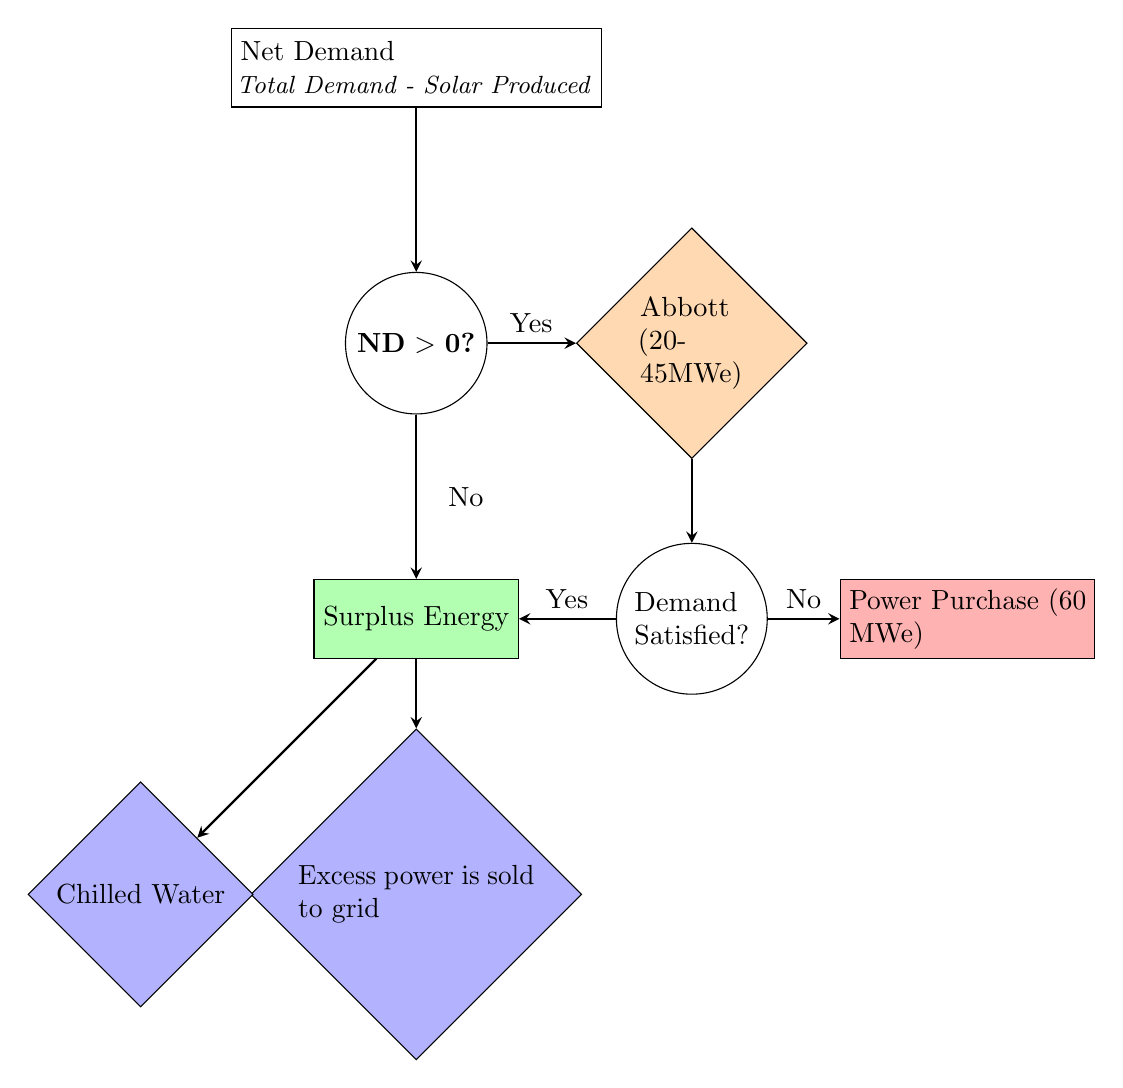
\begin{tikzpicture}[node distance = 3.5cm, auto, scale=0.25]
        \node (demand) [load] {Net Demand\\\small{\textit{Total Demand - Solar Produced}}};
        \node (ND) [decision, below of = demand] {\textbf{ND $>$ 0?}};
        \node (abbott) [supply, right of = ND] {Abbott (20-45MWe)};
        \node (isfull) [decision, below of = abbott] {Demand Satisfied?};
        \node (surplus) [extra, left of = isfull] {Surplus Energy};
        \node (purchase) [import, right of = isfull] {Power Purchase (60 MWe)};
        \node (buyback) [flexible, below of = surplus] {Excess power is sold to grid};
        \node (chilledwater) [flexible, left of = buyback] {Chilled Water};
  
        % \node (d1) [load, draw=none, below of = purchase] {\textbf{??}};
  
        \draw [arrow] (demand) -- (ND);
        \draw [arrow] (ND) -- node [text width = 1cm, midway, align=center] {No} (surplus);
        \draw [arrow] (ND) -- node [text width = 1cm, midway, above, align=center] {Yes} (abbott);
        \draw [arrow] (abbott) -- (isfull);
        \draw [arrow] (isfull) -- node [text width = 1cm, midway, above, align=center] {Yes} (surplus);
        \draw [arrow] (isfull) -- node [text width = 2cm, midway, above, align=center] { No } (purchase);
        \draw [arrow] (surplus) -- (chilledwater);
        % \draw [arrow] (purchase) -- (d1);
        \draw [arrow] (surplus) -- (buyback);
      \end{tikzpicture}
    
  \end{adjustbox}

  \captionof{figure}{The University of Illinois Energy Prioritization}

  \end{frame}
  % }

% \subsection{Abbott}
\section{Campus Energy Needs}
\subsection{Electricity}
\begin{frame}

	\begin{figure}
		\centering
		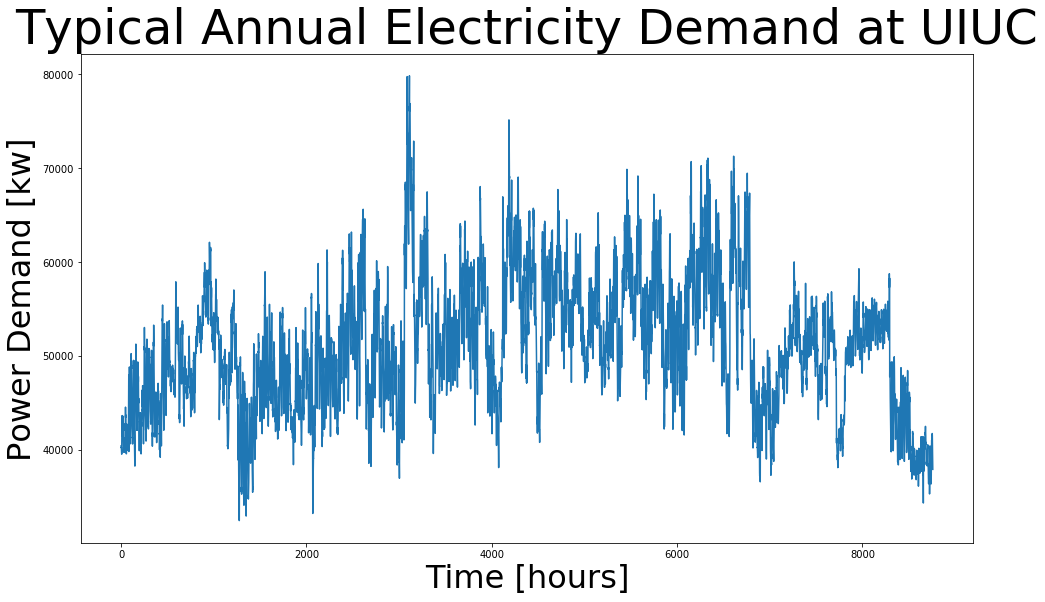
\includegraphics[width=0.9\textwidth]{./images/typical_demand.png}
		\caption*{The typical yearly electricity demand for UIUC. Average need is about 45 MWe, peaks near 80MWe.}
	\end{figure}

\end{frame}
\subsection{Steam}
\begin{frame}

	\begin{figure}
		\centering
		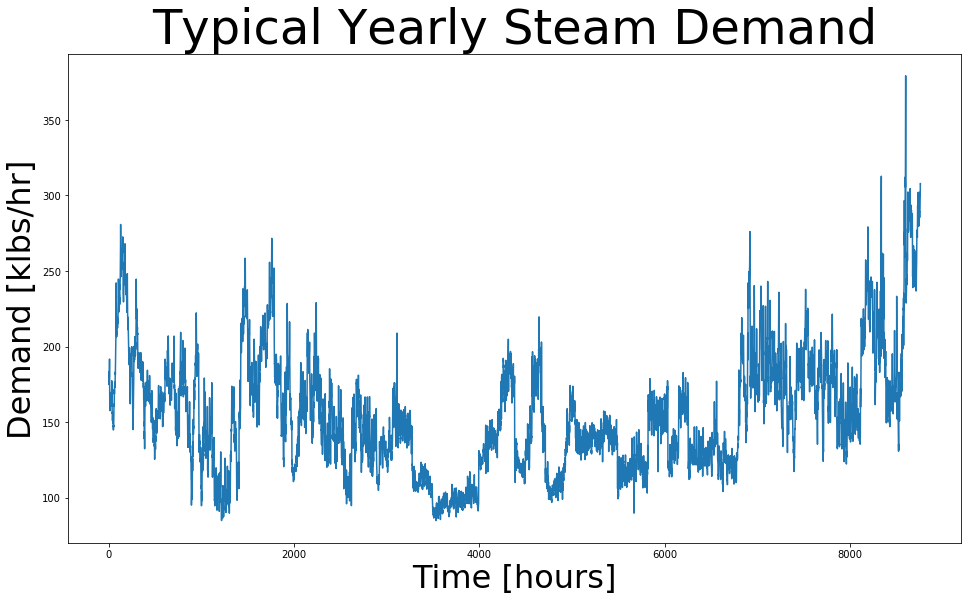
\includegraphics[width=0.9\textwidth]{./images/typical_steam.png}
		\caption*{The typical yearly steam demand for UIUC. Typical need is about 150 klbs/hr, peaks in the winter over 300klbs/hr.}
	\end{figure}

	
\end{frame}
\section{Systems}
\subsection{Abbott}
    \begin{frame}
  \frametitle{Abbott Power Plant}
  % a comment
        \begin{columns}
                \column[t]{5cm}
                Quick Facts \cite{noauthor_abbott_nodate}
                \begin{enumerate}
                    \item Cogeneration Plant (electricity is a ``byproduct'' of steam production).
                    \item Capable of producing 85 MWe (maximum capacity).
                    \item Capable of producing 800 Klbs/hr of steam (maximum capacity).
                \end{enumerate}
                \column[t]{5cm}
        \begin{figure}[htbp!]
        \begin{center}
      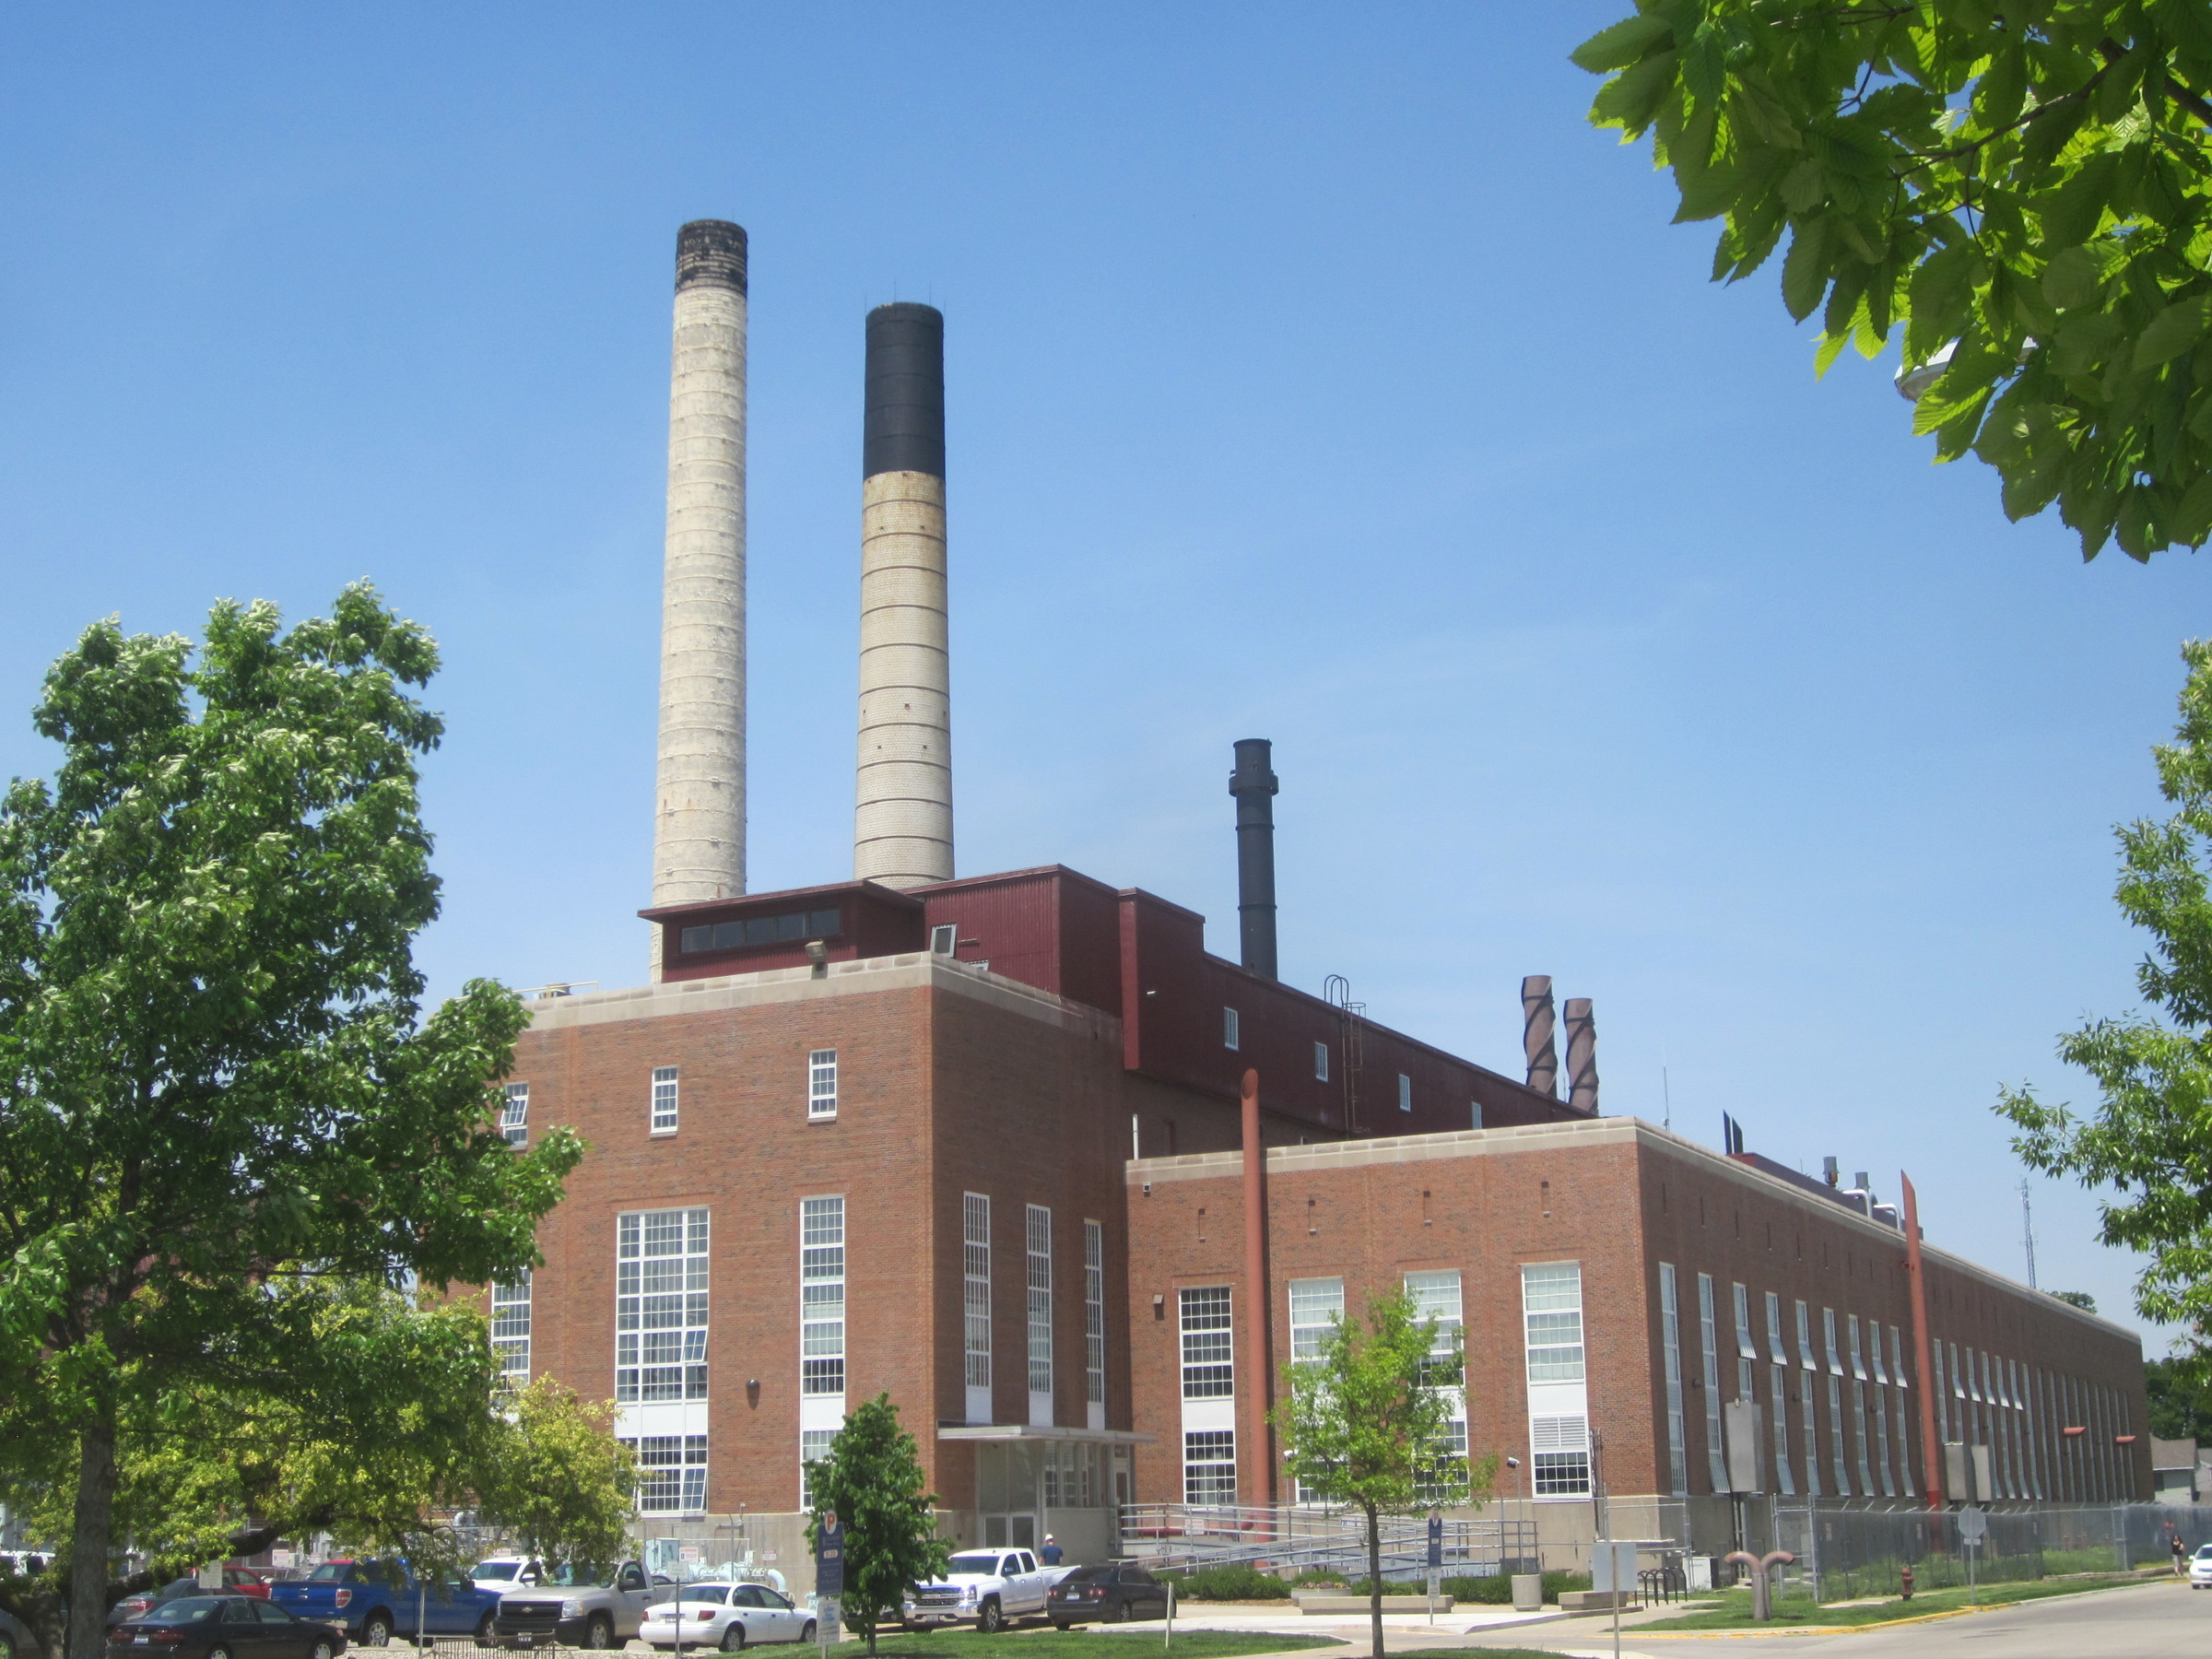
\includegraphics[height=4cm]{./images/abbott.jpg}
    \end{center}
          \caption*{South side of Abbott Power Plant.}
    \label{fig:abbott}
  \end{figure}
        \end{columns}
\end{frame}



\subsection{Solar Farm}
\begin{frame}
	
\begin{columns}
	\column[t]{5cm}
	Quick Facts \cite{white_solar_2017}
	\begin{itemize}
		\item Lifetime capacity factor of 16.8\%. 
		\item Rated to produce 4.8 MWe
		\item Soon to be expanded to 12.1 MWe
	\end{itemize}
	\column[t]{5cm}
	\begin{figure}
		\centering
		\label{fig:solarfarm}
		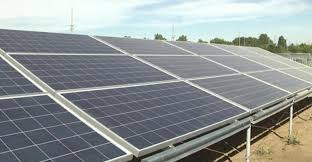
\includegraphics[width=0.8\textwidth]{./images/solarfarm.jpeg}
		\caption*{UIUC Solar Farm}
	\end{figure}
\end{columns}
	\begin{figure}
		\centering
		\label{fig:solardata}
		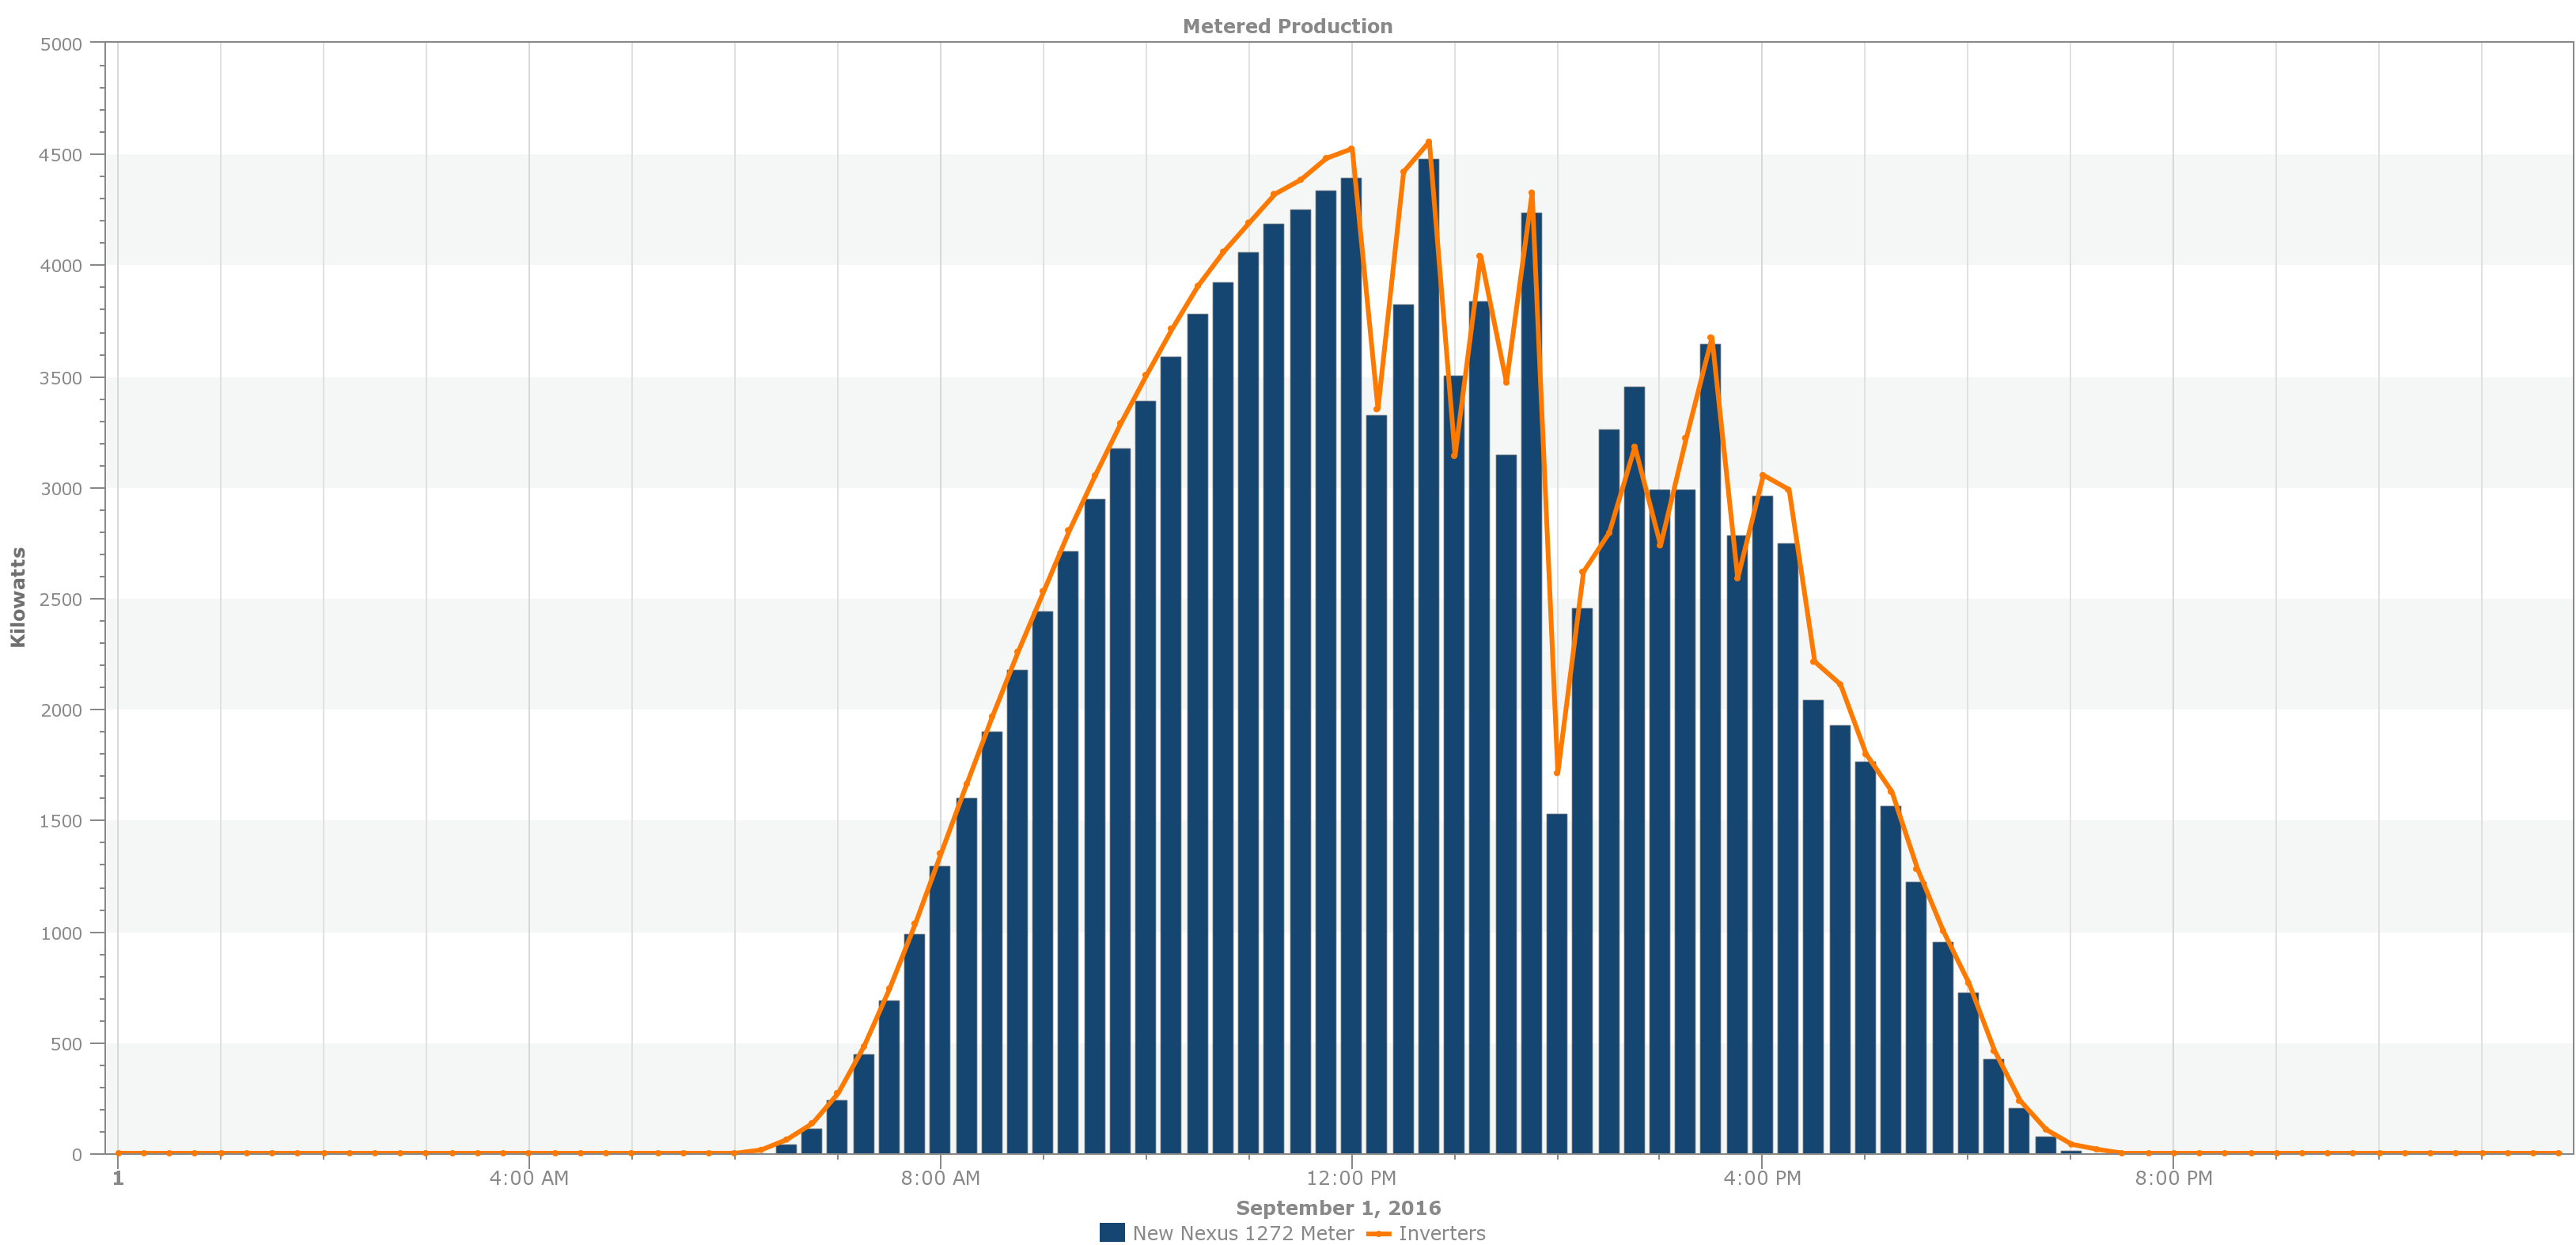
\includegraphics[width=0.75\textwidth]{./images/actual_solarfarm_9-1-2016.png}
		\caption{Actual solar farm data from AlsoEnergy \cite{alsoenergy_university_2019}}
	\end{figure}
\end{frame}

\begin{frame}
	\begin{figure}
		\centering
		\label{fig:typical_solar}
		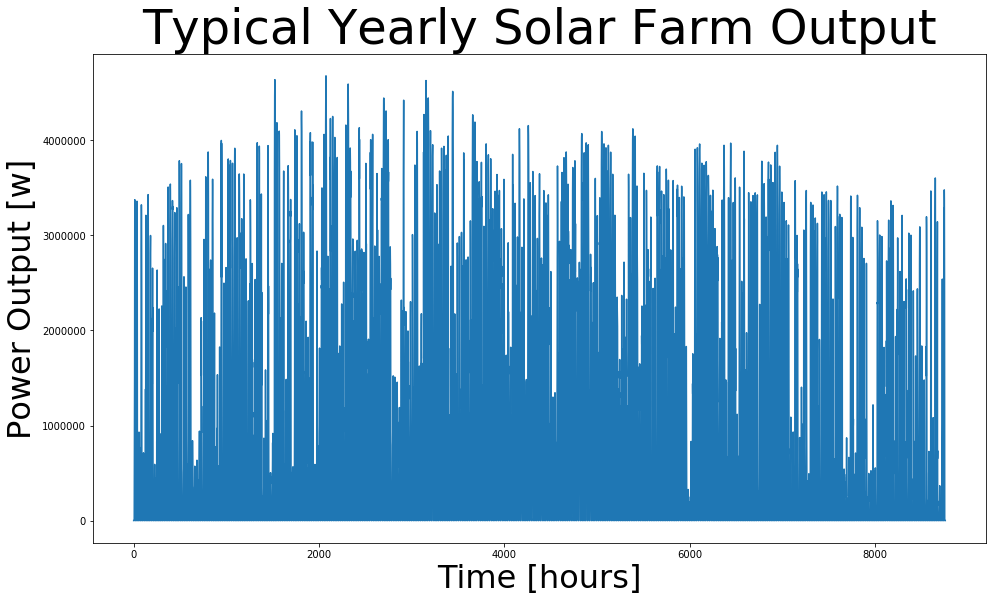
\includegraphics[width=0.9\textwidth]{./images/typical_solarpower.png}
		\caption{The typical power output of the UIUC solarfarm over a year.}
	\end{figure}
\end{frame}
\subsection{Power Purchase Agreement}
\begin{frame}
\Large{Power Purchase Agreements}\\


Quick Facts \cite{breitweiser_wind_2016}:

\begin{itemize}
	\item Power purchase agreement (PPA) with Rail Splitter Wind Farm
	\item PPA requires UIUC to buy 8.6\% of the energy produced by the wind farm.
	\item Fixed price of 4 cents/KWh
	\item Sometimes sold back at loss.\\
	e.g. A windy night when demand is low but the wind farm is producing a lot of electricity.
\end{itemize}
	
\end{frame}
\subsection{Chilled Water}
\begin{frame}

	\Large{Chilled Water}\\

	Quick facts \cite{noauthor_campus_nodate}:
	\begin{itemize}
		\item The energy consumption from chilled water is felt as electricity* demand.
		\item The only method of energy storage on campus. 
	\end{itemize}

	\small{*There are also steam driven chillers that are not currently being used.}
\end{frame}
\section{Current Work}
	
\begin{frame}
\large Current Work\\

	\begin{itemize}
		\item Finding the optimal size of a reactor to minimize the cost of electricity and steam. \\
                \item The method will use RAVEN (Rabiti, INL), and will be based on a paper 
                        \cite{baker_optimal_2018} that sized a reactor for a 
                        similar grid system.
	\end{itemize}
        \begin{figure}
                \centering
                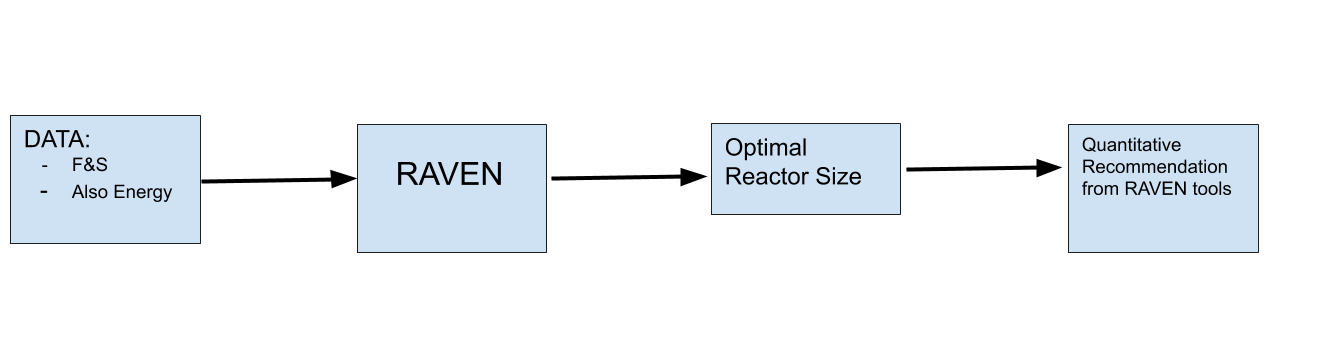
\includegraphics[height=0.5\textheight]{./images/flow.png}
                \caption{Work Plan.}
        \end{figure}
\end{frame}

\begin{frame}
        F\&S intends to retire the coal boilers by 2030 and replace them with 
        ``Developing Technologies,'' according to the Utilities Master plan 
        \cite{affiliated_engineers_inc_utilities_2015}. Without new 
        technologies available, the current plan is to replace this capacity 
        with  more PPAs and natural gas 
        \cite{affiliated_engineers_inc_utilities_2015}. However, small nuclear 
        power was mentioned as a possible ``developing technology'' which could 
        be considered if ready in time. 

	\begin{figure}
		\centering
		\label{fig:masterplan}
		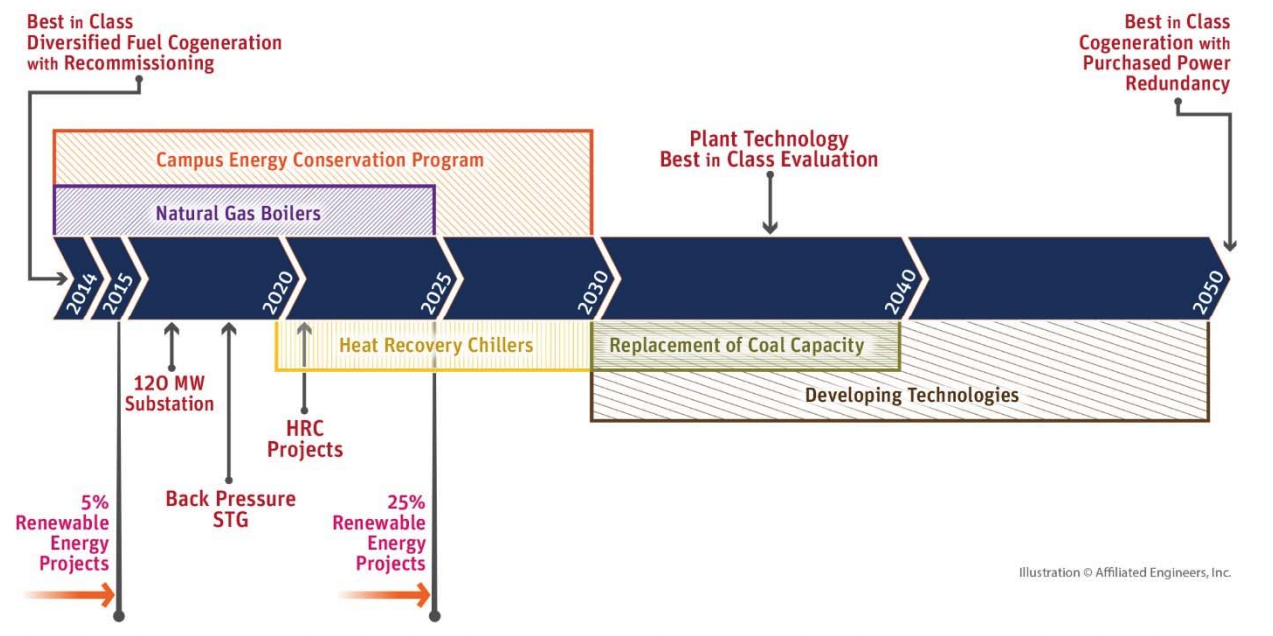
\includegraphics[width=0.75\textwidth]{./images/masterplan.png}
		\caption{Current trajectory suggests that campus should ``Re-evaluate and apply best of industry energy supply utilizing future advanced
technology and innovations for plant repowering in the 2030-2040 time frame.'' 
                \cite{affiliated_engineers_inc_utilities_2015}.}
	\end{figure}
\end{frame}

% \begin{frame}
  \frametitle{Acknowledgement}
        Acknowledgements should include both people who helped and funding 
        streams. If you are funded by an NEUP grant, that number usually goes 
        here. .
\end{frame}

%%--------------------------------%%
%%--------------------------------%%
\begin{frame}[allowframebreaks]
  \frametitle{References}
  \bibliographystyle{plain}
  {\footnotesize \bibliography{bibliography.bib} }

\end{frame}

%%--------------------------------%%


\end{document}



